\chapter {Results/ Findings}
\label{label10}


The results section presents the main findings of your research. Report all relevant results concisely and objectively, in a logical order. That gives your reader a clear idea of exactly what you found and keeps the data itself separate from your subjective analysis. Any evaluation of the findings should be discussed in the next section.

This section may contain visual elements accompanied by text. In quantitative research, it’s often helpful to include graphs, charts, tables, etc., but only if they are directly relevant to your results. Give these elements clear, descriptive titles and labels so that your reader can easily understand what is being shown (use numbering and caption title as recommended). 

Tables must be as simple as possible. Use numbers and title headings for each one. 
See the example below:


\begin{table}[!h]
\caption{Enrollment in local colleges, 2005}
\begin{center}
{\begin{tabular}{@{}cccc@{}} \toprule  College & New students & Graduating students & Change\\
 \midrule
& \textit{Undergraduate} & & \\
Cedar University & 110 & 103 & +7 \\
Elm College & 223 & 214 & +9\\
Maple Academy & 197 & 120 & +77\\ 
&  \textit{Graduate} & &     \\
Cedar University & 24 & 20 & +4 \\
Elm College & 43 & 53 & -10\\
Maple Academy & 3 & 11 & -8\\
 \midrule
Total & 600 & 521 & 79\\
\bottomrule
\end{tabular}}
\end{center}
\label{tab02}
\end{table}


Use the word “Figure” for images, diagrams and charts. Use numbers and title headings for each one. 
See the example below:

\begin{figure}[!ht]
\centering
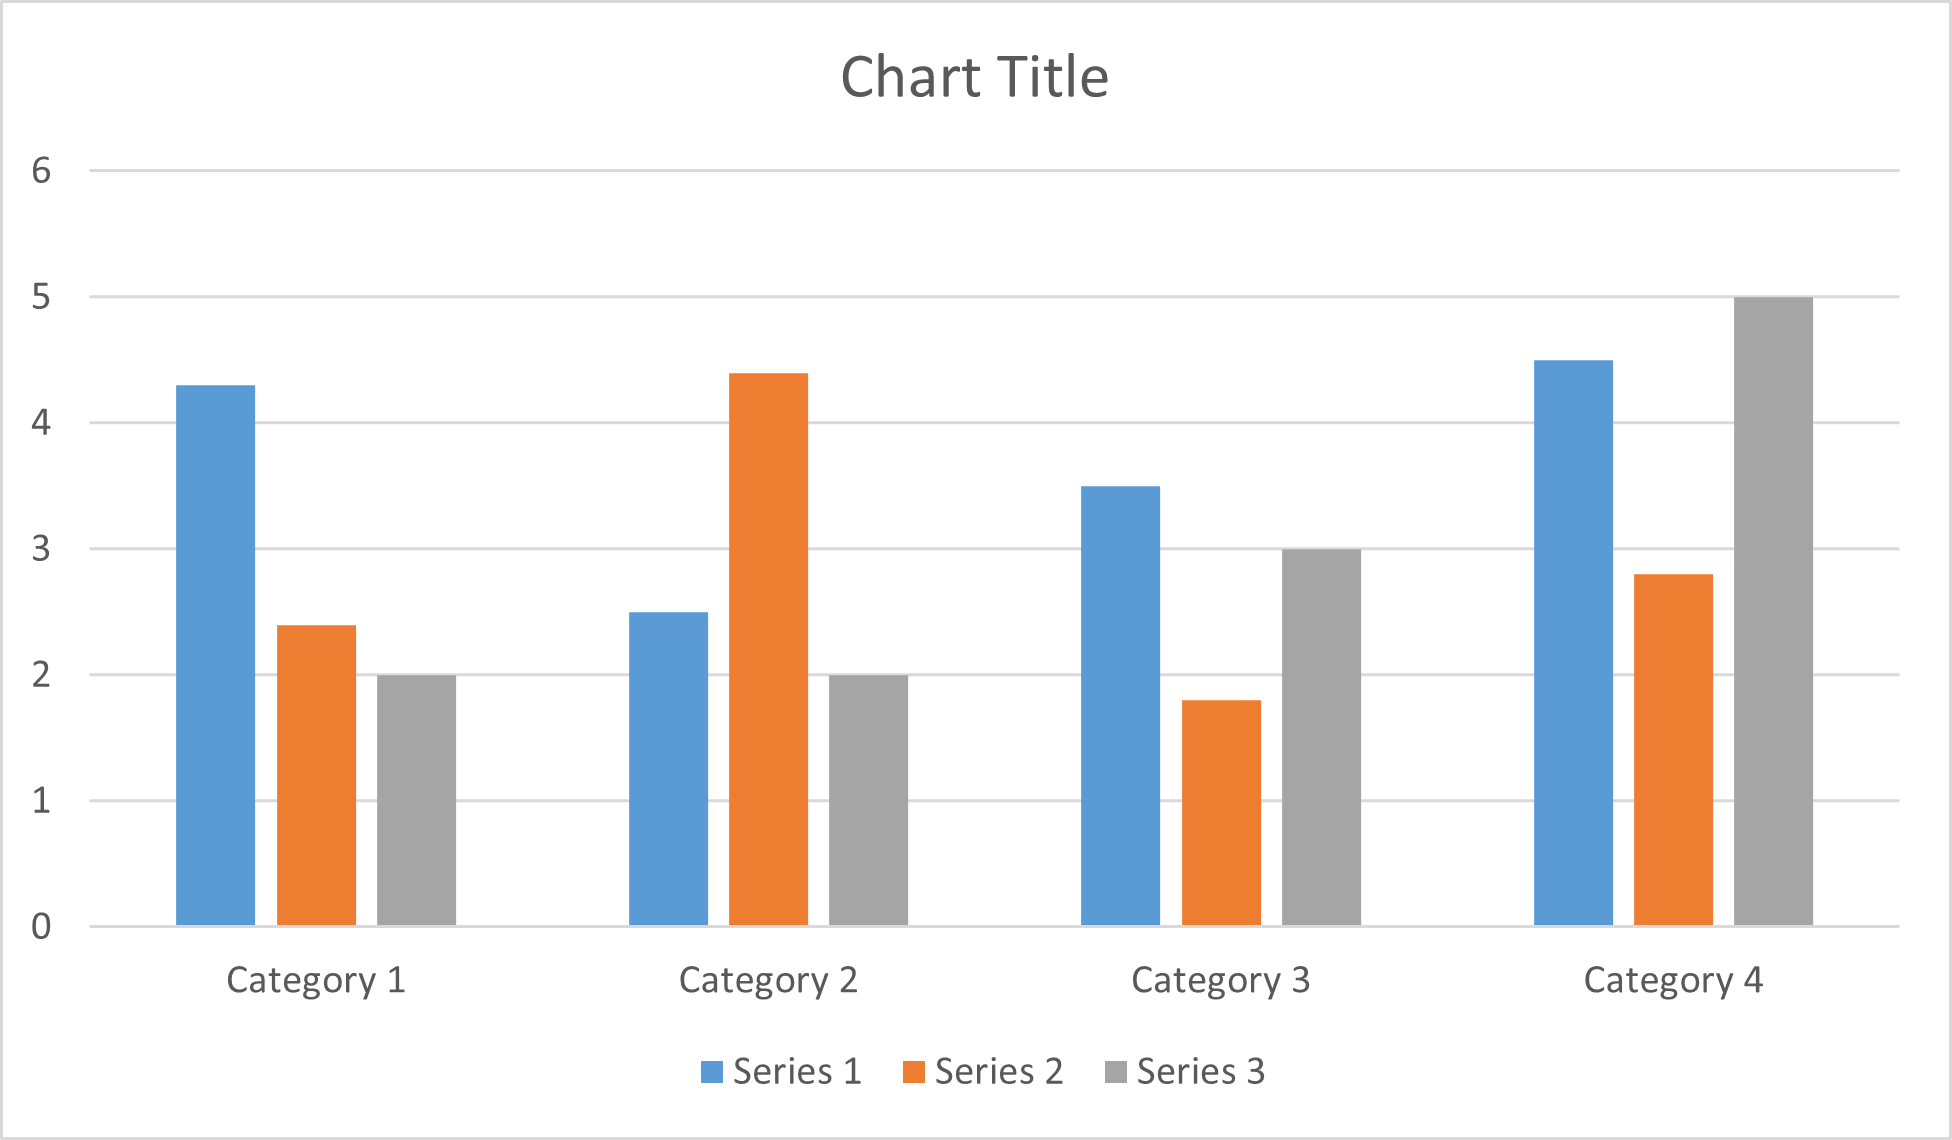
\includegraphics[width=\columnwidth]{figures/Chapter3/Chart Example.png}
\caption{Enrollment in local colleges, 2005}
\label{Fig2}
\end{figure}


\section{Section}
\label{label11}
 

\section{Section}
\label{label12}

\section{Summary}
\label{label13}